\ylDisplay{Ring ja ellips} % Ülesande nimi
{Tundmatu autor} % Autor
{lõppvoor} % Voor
{2015} % Aasta
{P 9} % Ülesande nr.
{3} % Raskustase
{
% Teema: Valgusõpetus
\ifStatement
Juuresoleval joonisel on kujutatud ring ja sellest koondava läätse poolt tekitatud kujutis. Leidke läätse keskpunkt, optiline peatelg ja fookus.
\begin{center}
	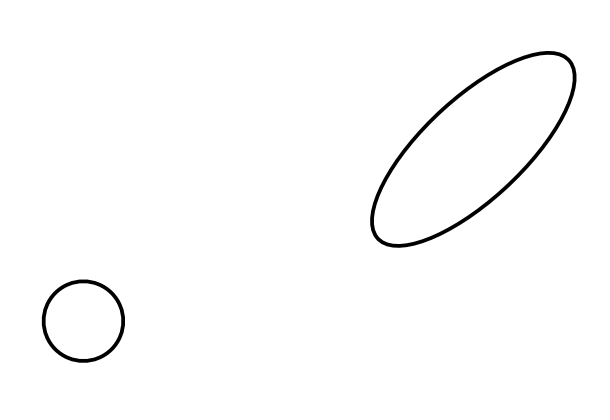
\includegraphics[width=0.5\linewidth]{2015-v3p-09-yl.PNG}
\end{center}
\fi
\ifHint
Läätse keskpunkti leiame kui ringile ja ellipsile tõmmatud puutujate lõikepunkti (puutepunktid peavad olema originaali-kujutise paarid ning neid ühendavad sirged peavad läbima läätse keskpunkti (sirged jooned joonisel).
\fi
\ifSolution
Läätse keskpunkti $O$ leiame kui ringile ja ellipsile tõmmatud puutujate lõikepunkti (puutepunktid peavad olema originaali-kujutise paarid ning neid ühendavad sirged peavad läbima läätse keskpunkti (sirged jooned joonisel). Läätse tasandi leidmiseks valime ringil kaks punkti $A$ ja $B$ ning leiame nende kujutised ellipsil sirgete $AO$ ja $BO$ ning ellipsi lõikepunktidena, olgu need $A'$ ja $B'$ , vt joonis. Kui originaal on ringi kahest lõikepunktist see, mis asub läätsest kaugemal, siis kujutis tuleb valida kahest lõikepunktist see, mis on läätsele lähemal (ja vastupidi), sest tõeline kujutis on pööratud tagurpidi. Kiir $AB$ peab murduma läätses kiireks $A'B'$ , murdepunkt annab meile punkti $L$ läätsel ning sirge $OL$ on läätse tasandiks. Optilise peatelje $o$ leiame sirgele $OL$ punktist $O$ tõmmatud ristsirgena. Fookuse leidmiseks tõmbame punktist $A$ kiire, mis on paralleelne $o$-ga ja murdub läätsel punkti $A'$ läbivaks kiireks, lõikepunkt $o$-ga annab fookuse $F$.
\begin{center}
	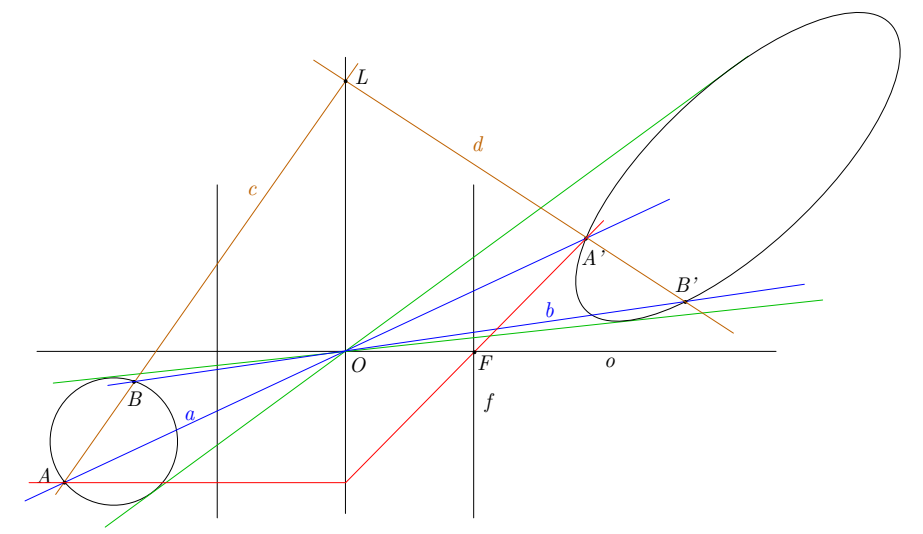
\includegraphics[width=0.5\linewidth]{2015-v3p-09-lah.PNG}
\end{center}
\fi
}
